\subsection{Catálogo de componentes}
El catalogo de componentes y plantillas es una herramienta de gestión
de conocimiento que permite a los integrantes de un equipo compartir,
reutilizar y colaborar en la creación de estándares para una mayor
eficiencia en el desarrollo de modelos de IA. Los componentes son
elementos que representan pequeñas funcionalidades dentro de un
proyecto que pueden ser reutilizados de una forma sencilla. Las plantillas 
por otro lado son estructuras más complejas. Estas pueden agrupar varios componentes, 
configuraciones y reglas de negocio. Ademas, cada una de ellas están organizadas dentro de una 
temática específica. A todos estos elementos los hemos
denominado bajo el nombre de STAC (Simple Tecnalia AI Components).\medskip

\subsubsection{Adaptación del diseño atómico}
La metodología de diseño atómico es una técnica que se basa en la
creación de componentes que puedan ser reutilizados en diferentes partes
de un proyecto. En el desarrollo de modelos de IA el posible adaptar
esta técnica para crear componentes que representen funcionalidades
específicas, como el preprocesamiento de datos, la selección de
características, la evaluación de modelos, entre otros.\medskip

Como se ha mencionado anteriormente, los componentes se dividen
a su vez en multitud de categorías (atómicos, moleculares, organismos, plantillas, etc.).
Esta división tiene sentido dentro de su concepción original pero,
en el caso de los modelos de IA, la división de los componentes se puede hacer
de una forma más sencilla, ya que en el caso de la investigación en IA, una
abstracción más sencilla puede ser más útil para los investigadores. 
Esta abstracción permitiría reducir la complejidad de los componentes y
facilitar su reutilización en diferentes proyectos. Es por
ello que se propone una división de los componentes en tres categorías:

\begin{itemize}
    \item \textbf{Componentes atómicos:} son los componentes más sencillos
    que representan una funcionalidad específica.
    \item \textbf{Componentes compuestos:} estos componentes agrupan
    varios componentes atómicos para realizar una funcionalidad más
    compleja.
    \item \textbf{Plantillas:} estructuras de proyectos completan que buscan
    solucionar un problema específico utilizando una técnica concreta. Están
    formadas a su vez por componentes compuestos y atómicos. Además, las
    plantillas también agrupan configuraciones, reglas de negocio y
    diversas integraciones con otros sistemas.
\end{itemize}

Todos los componentes y plantillas se almacenan en un repositorio
compartido, donde los integrantes del equipo pueden colaborar en la
creación de nuevos componentes y plantillas, así como en la mejora de
los existentes.

\subsubsection{Estructura del sistema de componentes}
La arquitectura que se ha decidido implementar para el sistema de componentes
es conocida como monorepo multi-paquete. Un monorepo es una práctica de 
desarrollo de software donde todos los proyectos relacionados 
se almacenan en un único repositorio de código fuente. Esto significa que en 
lugar de tener múltiples repositorios para cada uno de los componentes, todo se 
mantienen en un único lugar. Por otro lado, que sea multi-paquete significa que
que los diferentes elementos del monorepo se organizan mediante paquetes de
software, lo que facilita su distribución de forma independiente. Este tipo de 
arquitectura cuenta con varias ventajas, entre las que se encuentran:

\begin{itemize}
    \item \textbf{Facilidad de gestión:} Tener todo en un solo lugar simplifica la gestión 
    del código, las dependencias y las versiones. No es necesario alternar entre
    diferentes repositorios para hacer cambios o resolver problemas.
    \item \textbf{Consistencia:} Todos los proyectos dentro del monorepo pueden seguir 
    las mismas convenciones, estructura de carpetas, y configuraciones, 
    lo que garantiza una mayor consistencia en el código. Esto permite que el código
    sea más fácil de mantener a largo plazo.
\end{itemize}

Uno de los principales problemas que puede surgir al utilizar un monorepo es la
complejidad que puede acarrear la organización de las diferentes carpetas, ya
que al tener todo en un solo lugar, la cantidad de archivos puede llegar
a ser muy grande y contar con un nivel de anidamiento muy profundo. Para evitar este
problema, se ha decidido tomar una estructura de carpetas basada en 
\textit{Screaming Architecture} \cite{Screaming}, una arquitectura de software que busca anteponer la
lógica de negocio sobre las partes técnicas del sistema. En este caso, nuestra lógica de
negocio se relaciona en torno al problema que se busca resolver, es decir, los diferentes 
tipos de problemas de series temporales.\medskip

\begin{figure}[!h]
    \dirtree{%
        .1 /components.
        .2 /TimeSeries-Forecasting.
        .3 /Data-Ingestion.
        .4 ingestion-component-1.
        .4 ingestion-component-2.
        .3 /Data-Processing.
        .4 processing-component-1.
        .3 /Models.
        .4 model-component-1.
        .2 /TimeSeries-Classification.
        .3 /Data-Processing.
        .4 processing-component-2.
        .3 /Metrics.
        .4 metric-component-1.
        .2 /TimeSeries-AnomalyDetection.
        .3 /Data-Processing.
        .4 processing-component-3.
    }
    \caption{Ejemplo de estructura de carpetas basada en Screaming Architecture.}
    \label{fig:screaming-arch}
\end{figure}

La figura \ref{fig:screaming-arch} muestra un ejemplo simplificado de la estructura
de carpetas del proyecto. Por cada uno de los diferentes problemas, se ha creado una 
carpeta principal, que a su vez contiene diferentes subcarpetas que agrupan los 
diferentes componentes dentro de cada una de las temáticas (procesamiento, modelo, métricas). 
En caso de que se necesite añadir un nuevo componente, simplemente se crea una nueva
carpeta dentro de la temática correspondiente. Por ejemplo, tomando la temática \textit{preprocesamiento de datos}
dentro de clasificación, se buscaría la carpeta \textit{Data-Processing} dentro de la sección
\textit{TimeSeries-Classification} y en caso de no existir, se crearía una nueva , y dentro de ella 
se añadiría el nuevo componente. \medskip

Lo que se consigue con este enfoque es que cada uno de los diferentes problemas cuente con una 
estructura similar pero que a su vez tengan la posibilidad de incluir temáticas propia. En la
figura \ref{fig:screaming-arch} se puede ver como cada uno de los problemas cuenta con componentes
de procesamiento de datos, pero que a su vez, hay algunos de ellos que cuentan con componentes
específicos de modelos o métricas. Esto se puede deber a que cada uno de los problemas tiene
una necesidades específicas o que no se han encontrado componentes que se puedan reutilizar
en este momento.\medskip

\subsubsection{Empaquetado de componentes}
La idea de los componentes es que sean fácilmente integrables en cualquier
proyecto de una forma sencilla. Para ello, se ha decidido empaquetar cada
componente de forma independiente y distribuirlos dentro de un repositorio
privado, de forma que se puedan instalar utilizando pip o cualquier otro 
gestor de paquetes como poetry.\medskip

Dentro de nuestro caso de uso, queremos tener la posibilidad de instalar
solo aquellos componentes que necesitemos en cada momento, sin tener que
descargarnos todo el contenido del repositorio. Esto es especialmente 
importante ya que las dependencias de las librerías de IA pueden llegar a
ser muy pesadas. A su vez, también se quiere que todos nuestros componentes
hereden del mismo nombre de paquete, para que se puedan utilizar de una forma
transparente a la hora de importarlos en un proyecto. Es decir, si tenemos por
ejemplo un componentes de ingesta de datos llamado \textit{get\_data} y otro de 
visualización que imprime una gráfica llamado \textit{show\_graph}, la forma de 
importarlo en un proyecto real sería la que se muestra en la figura \ref{fig:import-components}.

\begin{figure}[!h]
    \begin{lstlisting}[language=Python]
        $ pip install stac-show-graph stac-get-data

        >>> from stac.visualization.show_graph import show_graph
        >>> from stac.data_ingestion.get_data import get_data
        >>> data = get_data()
        >>> show_graph(data)
    \end{lstlisting}
    \caption{Ejemplo de importación de componentes.}
    \label{fig:import-components}
\end{figure}

Para conseguir este efecto es necesario comprender como funciona el empaquetado
de librerías en Python. En Python, un paquete es una carpeta que contiene, por lo menos,
un archivo \textit{\_\_init\_\_.py} y un \textit{pyproject.toml} o \textit{setup.py}. 
La forma en la que se importan los paquetes es a través de un sistema de rutas por archivos, 
donde se toma la ruta hacia el paquete desde el directorio raíz del proyecto. En este caso,
si queremos que todos nuestros componentes se importen desde \textit{stac}, es necesario que
el código de cada uno se encuentre dentro de una carpeta llamada \textit{stac}, que a su vez
contenga una carpeta con el nombre de la categoría del componente sin ningún \textit{\_\_init\_\_.py} 
en su interior, ya que no queremos que se comporte como un paquete sino como una ruta.
Dentro de esta, se crear una carpeta con el nombre del componente y se añadirá el código 
del componente. En la figura \ref{fig:min-package} se puede ver 
como es el contenido de cada componente y la estructura de carpetas que se debe seguir.\medskip 

\begin{figure}[!h]
    \dirtree{%
        .1 /component-name.
        .2 pyproject.toml.
        .2 /stac/component-category/component-name.
        .3 \_\_init\_\_.py.
    }
    \caption{Estructura mínima de un componente empaquetado.}
    \label{fig:min-package}
\end{figure}

Esta estructura se tiene que repetir para cada uno de los componentes que se quieran
añadir al repositorio. No obstante, y aprovechando que cada componente está separada
en un proyecto independiente, se pueden añadir más utilidades como tests, documentación
o ejemplos de uso. Como estamos utilizando poetry para gestionar las dependencias, y
las configuraciones globales del proyecto, también se van a añadir sus archivos 
correspondientes.\medskip

\begin{figure}[!h]
    \dirtree{%
        .1 /component-name.
        .2 README.md.
        .2 pyproject.toml.
        .2 poetry.lock.
        .2 Makefile.
        .2 /tests.
        .2 /stac/component-category/component-name.
        .3 \_\_init\_\_.py.
    }
    \caption{Estructura final de un componente empaquetado.}
    \label{fig:real-package}
\end{figure}

Este empaquetado puede parecer tedioso si se tiene que hacer manualmente, pero en
futuras secciones veremos como se ha automatizado este proceso para que sea lo más
sencillo posible. Es muy importante que la estructura sea la descrita para optimizar
la experiencia de desarrollo de los integrantes del equipo.

\subsubsection{Sistema de plantillas}
La herramienta que hemos utilizado para la creación de plantillas es Cookiecutter \cite{Cookiecutter}.
Cookie\-cutter es una utilidad para la generación de proyectos que te permite inicializar
un proyecto a partir de plantillas predefinidas. Funciona siguiendo un principio 
básico: en lugar de empezar un nuevo proyecto desde cero y tener que configurar 
todo manualmente, puedes usar una plantilla predefinida que ya incluya la estructura 
de directorios, archivos básicos, configuraciones iniciales, y cualquier otro 
componente necesario para tu proyecto.\medskip

La razón de la elección de Cookiecutter es por su facilidad de uso, ya que
al utilizar el sistema de plantillas Jinja2 \cite{Jinja}, se pueden añadir variables a los
archivos de la plantilla que se sustituirán por valores concretos al inicializar
el proyecto. Este sistema de plantillas es muy conocido especialmente ente los
desarrolladores de Python, ya que es ampliamente utilizado por otros frameworks
web como Django. Además, Cookiecutter cuenta con una gran cantidad de plantillas
predefinidas que se pueden utilizar de forma gratuita, lo que puede ser muy útil
a la hora de incorporar las primeras plantillas al repositorio.\medskip

Esto es especialmente útil en entornos donde necesitas crear múltiples proyectos 
con una estructura similar donde puede haber proyectos con requisitos comunes, 
como la configuración de un marco de trabajo específico, estructura de directorios 
estándar, o incluso configuraciones de pruebas y documentación. Además, en nuestro
caso son especialmente útiles ya que contamos con tres situaciones en las que tener
una plantilla puede ser muy útil:

\begin{itemize}
    \item \textbf{Creación de plantillas para problemas específicos:} este es el caso
    principal de el uso de plantillas. Cada una de las plantillas se crea para resolver
    un problema específico con una técnica concreta. Por ejemplo, una plantilla para
    clasificación de series temporales con redes neuronales recurrentes.
    \item \textbf{Creación de nuevos componentes:} en caso de que se quiera añadir
    un nuevo componente al repositorio, se puede utilizar una plantilla que contenga
    la estructura de carpetas y los archivos necesarios para empaquetar el componente.
    Como hemos mencionado anteriormente, la automatización es un aspecto clave para 
    incentivar las contribuciones.
    \item \textbf{Creación de nuevas plantillas:} la estructura base de las plantillas
    al igual que los componentes es fácilmente reutilizable, ya que ciertos archivos de
    configuración o de documentación pueden ser compartidos entre diferentes plantillas. Por
    lo que se pueden crear nuevas que contengan estos archivos y asi automatizar el
    proceso de creación. 
\end{itemize}


Estas plantillas se almacenan de la misma forma que podemos ver en la figura
\ref{fig:screaming-arch} pero sustituyendo los componentes por las plantillas.
En principio, la estructura de las plantillas puede variar en gran medida entre
ellas, ya que cada una de ellas busca resolver un problema específico. No obstante,
hay una serie de directrices obligatorias que se deben seguir para garantizar el
correcto funcionamiento de las plantillas:

\begin{itemize}
    \item \textbf{Automatización de instalación y lanzamiento:} todas las plantillas
    deben contar con un \textit{Makefile} que permita la instalación de las dependencias y
    el lanzamiento de la aplicación de forma sencilla. Por convención, el comando
    de instalación se llamará \textit{make install} y el de lanzamiento \textit{make train}.
    Es muy importante que estos comandos estén presentes en todas las plantillas para
    garantizar que con solo dos comandos y sin necesidad de consultar la documentación
    específica de cada plantilla se pueda poner en marcha el proyecto.
    \item \textbf{Documentación:} todas las plantillas deben contar con una documentación
    clara y detallada sobre el uso de la plantilla. Esta documentación se debe almacenar
    en un archivo \textit{README.md} en la raíz de la plantilla y debe contener una descripción
    general de la plantilla, disponer del comando de descargo para token de acceso y ssh,
    un listado de los archivos que se generan y un listado de las etiquetas que se han
    utilizado para indexar en el sistema de búsqueda.
\end{itemize}

\subsubsection{Integración continua y despliegue continuo}
Dentro de equipos de trabajo donde hay un número elevado de integrantes, es
importante no solo tener una buena organización del código, sino también
contar con un sistema de CI/CD que asegure los diferentes procesos. En este
caso es especialmente crítico ya que los componentes son utilizados por
diferentes investigadores en diferentes proyectos, por lo que un fallo en uno de
los componentes puede afectar a un gran número de proyectos.\medskip

Para la implementación se ha utilizado GitLab CI, con una distribución de 
tres fases: 
\begin{itemize}
    \item \textbf{test:} en esta fase se ejecutan los test de cada uno de los componentes
    para comprobar que no hay errores en el código. En caso de que haya errores, se
    notifica y se detiene el proceso. Estos test funcionan mediante el uso de Pytest \cite{Pytest},
    una librería de Python que permite la creación de test unitarios de una forma sencilla.
    \item \textbf{pages:} en esta fase se extraen todos los archivos de documentación que están 
    conformados por los \textit{README.md} y \textit{README.mdx} de las carpetas de componentes. 
    Una vez extraído se genera una página web estática con toda la documentación del proyecto.
    \item \textbf{deploy:} en esta fase se comprueba que paquetes es necesario desplegar y en caso
    de que haya cambios, se despliegan las nuevas versiones de los paquetes. Estas versiones se despliegan
    bajo una nuevo versión lo que se mantienen los paquetes anteriores para evitar problemas de compatibilidad.
\end{itemize}


Estas fases se ejecutan en diferentes momentos, y al estar la rama principal bloqueada
por defecto, es necesario crear una rama con las nuevas funcionalidades y/o modificaciones
y hacer una petición de \textit{merge} a la rama principal. En este momento se ejecutan las fases
de test y docs, para comprobar que no hay errores en el código y que la documentación
se puede generar correctamente, aunque esta última no se despliega hasta que se haya
aceptado la petición de merge. En caso de que se acepte la petición de merge, se ejecuta
la fase de deploy. Existen usuarios que excepcionalmente pueden realizar modificaciones
sobre la rama principal, pero solo en caso de que sea necesario y no como una práctica
habitual. 

\begin{figure}[!h]
    \centering
    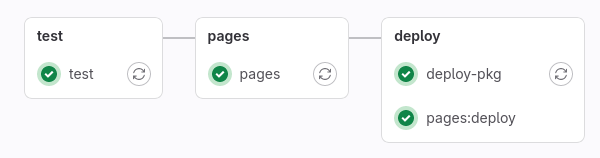
\includegraphics[width=0.8\textwidth]{component_pipe.png}
    \caption{Ejecución de una \textit{pipeline} completa.}
    \label{fig:component-pipeline}
\end{figure}
